% interactcadsample.tex
% v1.03 - April 2017

\documentclass[12pt]{interact}
\usepackage{fix-cm}
\usepackage{fontspec}
\setmainfont{Latin Modern Roman}

\usepackage{graphicx}% For including graphics
\graphicspath{{figures_png/}{figures/}}% Figures live in ./figures/ next to main.tex (Overleaf-friendly)
\usepackage{booktabs}% Required by the publication tables below
\usepackage{subfigure}% Support for small, `sub' figures and tables
%\usepackage[nolists,tablesfirst]{endfloat}% To `separate' figures and tables from text if required
\usepackage{polyglossia}
\setmainlanguage{english}
\setotherlanguage{ukrainian}
\newfontfamily\ukrainianfont{FreeSerif}

\usepackage{natbib}% Citation support using natbib.sty
\usepackage{hyperref}
\hypersetup{
  colorlinks=true,
  citecolor=blue,
  linkcolor=blue,
  urlcolor=blue,
  filecolor=blue
}
\bibpunct[, ]{(}{)}{;}{a}{}{,}% Citation support using natbib.sty
\renewcommand\bibfont{\fontsize{10}{12}\selectfont}% Bibliography support using natbib.sty

\theoremstyle{plain}% Theorem-like structures provided by amsthm.sty
\newtheorem{theorem}{Theorem}[section]
\newtheorem{lemma}[theorem]{Lemma}
\newtheorem{corollary}[theorem]{Corollary}
\newtheorem{proposition}[theorem]{Proposition}

\theoremstyle{definition}
\newtheorem{definition}[theorem]{Definition}
\newtheorem{example}[theorem]{Example}

\theoremstyle{remark}
\newtheorem{remark}{Remark}
\newtheorem{notation}{Notation}
\usepackage{microtype}
\PassOptionsToPackage{hyphens}{url}
\urlstyle{same}
\renewcommand{\UrlFont}{\rmfamily}

\begin{document}

\articletype{Capstone Project}

\title{Speaking We in Wartime: Pronominal Deixis and National Address in Ukrainian Facebook Poetry, 2014–2025}

\author{
\name{Junyu Jiang\textsuperscript{a}and Amelia Glaser\textsuperscript{b}}
\affil{\textsuperscript{a}M.S. Computational Social Science, UC San Diego; \textsuperscript{b}Professor in Literature Department, UC San Diego}
}

\maketitle

\begin{abstract}

\end{abstract}

\begin{keywords}
Ukrainian Contemporary Poetry; Digital Humanities; Wartime Discourse; Pronominal Deixis; Within-Author Design
\end{keywords}

\section{Introduction}

Poets in Ukraine have long used verse as a way of describing the nation’s struggles. This practice has increasingly shifted online; following the outbreak of the war in Donbas in 2014, poets frequently engaged with themes of war, identity, and community. However, the full-scale invasion on 24 February 2022 came as a profound shock to Ukrainian society, including its literary community. Within days of the first missile strikes on Kyiv, poets were publishing short verse to their Facebook pages, initiating an ongoing public conversation among writers, readers, and editors \citep{glaser2024poetry}. The Contemporary Ukrainian Poetry Archive \citep{glaser2024archive} preserves this record. The significance of the Ukrainian case extends beyond mere textual preservation; it lies in the way the poets themselves have actively created a usable, time-stamped archive. These wartime conditions provide a critical analytical window to test how an existential crisis prompts the reconceptualization of community and collective belonging through specific grammatical mechanisms.

To explore these dynamics, we focus on pronominal deixis: the grammatical choices that position the speaker, addressee, and adversary in social and political space. Critical linguistics treats these deictic forms as a principal grammatical site where speech acts tie directly to personal and social identities \citep{muhlhausler1990pronouns}. Regarding the construction of national identity, \citet{anderson2006imagined} famously argues that the nation functions as an imagined community, a social construct continually flagged and reproduced through the routine, unreflective use of forms like ``we'' and ``our'' \citep{billig1995banal}. In this paper, we investigate whether the full-scale invasion changed the way Ukrainians describe collective identity and subjecthood, utilizing a large sample of poems from Facebook accounts to analyze how Ukrainian poets articulate these shifts.

We address two primary research questions. To isolate the immediate impact of the invasion and eliminate between-author confounding, both questions rely on a within-author design that treats each poet as their own control \citep{Hernn2016}.

\textbf{RQ1:} Do within-author rates of first-person (singular and plural) and second-person (singular and plural) pronouns shift at the corpus level across the 24 February 2022 invasion cutpoint?

\textbf{RQ2:} How are these deictic shifts distributed across individual authors? Does the aggregate corpus-level effect mask heterogeneous or countervailing trajectories among individual poets writing through the cutpoint?

\section{Literature Review}

\subsection{Pronouns as Political Grammar}
Within the pragmatic and critical-linguistic tradition, pronouns occupy a central place as the primary grammatical site of identity work \citep{muhlhausler1990pronouns}, and routine deictic flagging continually reproduces the nation as an unmarked background of everyday discourse \citep{billig1995banal}. \citet{wilson1990politically} offers a political-pragmatic account of how speakers deploy we and they to assign responsibility, signal solidarity, and demarcate political alignments. This polarization, formalized as the ideological square \citep{vanDijk2011}, manifests empirically in the distribution of first- and third-person plural pronouns across political genres. The corollary at the pronoun level is that observable shifts in 1PL frequency mark movement of the discursive boundary between in-group and out-group, not stylistic preference.
Several frameworks render these claims tractable for corpus analysis. The Deictic Space Model \citep{chilton2004analysing} anchors space, time, and modality to the speaker's deictic center and the in-group we, generating axes of us-here-now versus them-there-then—axes that apply directly to wartime verse, whose enemy is by definition geographically and morally distant. The Discourse-Historical Approach \citep{wodak2009the} formalizes the referential, predicational, and perspectivation strategies through which national sameness and difference are constructed, with pronominal deixis as the prototypical referential resource. \citet{reyes2011strategies} extends this apparatus to legitimization discourse, where the same pronominal framing of us-as-victims against them-as-threat performs argumentative work. \citet{petersoo2007what} shows that the deictic center of the national we routinely oscillates among multiple referents within a single text—the so-called ``wandering we''—while \citet{fina1995pronominal} models how pronominal choice indexes identity and solidarity in political discourse, supplying an analytic template adaptable to the persona work of wartime poetry. A further methodological consideration is that 1PL inclusivity, grammatically marked in some languages, is only pragmatically inferred in Ukrainian and Russian \citep{cysouw2003the, filimonova2005clusivity, helmbrecht2002grammar}; reference must therefore be reconstructed from context rather than read off morphology. Taken together, these frameworks specify how 1PL and 2P forms function as coordinates in a discursive field, but they do not specify which field. The Ukrainian wartime case, to which I turn next, supplies that content.

\subsection{Ukrainian Identity as Discursive Event}

Brubaker's program reconceptualizes ethnic and national identity as a contingent, variable process, which licenses reading pronoun choice as nation-making rather than nation-describing. Nationalism Reframed \citep{brubaker1996nationalism} introduces the triadic nexus of nationalizing state, national minority, and external homeland that has structured subsequent analyses of post-Soviet Ukrainian- Russian relations. In ``Beyond Identity,'' \citet{brubaker2000beyond} decomposes the term into identification, self-understanding, and commonality, and argues that ``identity'' reifies what is more usefully analysed as process. Ethnicity Without Groups \citep{brubaker2004ethnicity} recasts groupness itself as a contingent event, an achievement of categorization, mobilization, and discursive practice. The cognitive-linguistic extension of this argument \citep{brubaker2004ethnicity1} treats ethnicity, race, and nation as schemas through which actors parse experience, which warrants reading pronoun choice as an observable trace of category activation.

These conceptual moves find direct purchase in the Ukrainian record. Ukrainian nationhood has long been documented as a contested cultural construct rather than a primordial group, and ethno-nationalism remained a minority position among the titular nationality throughout the 1990s \citep{wilson1997ukrainian, wilson2000the}. \citet{kulyk2001the} brings the Brubakerian framework into Ukrainian studies, critiques its majority/minority assumption, and reformulates Ukrainian nationhood as discursive practice in post-Soviet ethnopolitics; \citet{kulyk2016national, kulyk2018shedding} show that the substantive content of being Ukrainian shifted after 2014, with ethnonational identifications recast rather than merely activated. For pronoun-level inference, this entails that the referent of a Ukrainian poet's ``we'' cannot be assumed stable across the 2014--2025 window; the referent is itself an object of contestation. If the category is contested, the further question is whether it is also internally multidimensional and time-varying.

The evidence indicates that it is. \citet{onuch2018capturing} decompose ethnicity into four measurable dimensions and show that substantive conclusions depend on which dimension is operationalized. Civic and
ethnolinguistic identifications are decoupled, and mixed identifications persist along the contact line \citep{popeleches2018identity, sasse2018war}. The predictive purchase of ethnolinguistic categories themselves varies over time \citep{kulyk2022imperfect}, and the civic Ukrainian nation can be read as
a generation-specific, performative accomplishment that crystallized under invasion \citep{onuch2022the}. Inference about pronominal address must therefore be situated against the sociolinguistic context from which the poetic corpus emerges. \citet{bilaniuk2005contested, bilaniuk2010language} provides the standard ethnographic account of Ukrainian--Russian bilingualism
and the politics of non-accommodation that prevailed before 2014; \citet{kulyk2024language} documents a historically sharp retreat of Russian from everyday Ukrainian life after 2022; \citet{popova2024russia} traces the strategic narratives circulating during the war; and \citet{plokhy2021the} situates these contemporary contests in the longue durée of Ukrainian state formation. A Ukrainian-language poetic corpus spanning 2014--2025 therefore cannot be read against a stable linguistic baseline, since the language of composition is itself part of what is shifting.

Three caveats qualify the use of this identification record as ground for inference about poetic grammar. First, the survey-based studies \citep{kulyk2016national, onuch2018capturing, kulyk2022imperfect} measure population-level identifications, not the grammatical practice of writers;
poets are not a representative sample of the surveyed population, and no claim of demographic generalizability is intended here. Second, on the reading developed by \citet{glaser2024poetry}, Facebook poetry in this period functions as circulating public discourse rather than individualized lyric
record. Poets in this archive operate as self-selected articulators of the national discursive field; their work is addressed to networked publics and recirculated within them. Their pronoun choices are accordingly more informative about that collective field than a representative corpus would be, not less, because they are produced under explicit discursive accountability. Third, it follows directly from \citet{billig1995banal} and \citet{petersoo2007what} that an identification shift should leave traces in routine pronominal practice. If banal national ``we''-flagging is itself a sensitive marker of sociopolitical context, then routine pronominal practice should register the shifts visible in the post-2014 and post-2022 windows.

\subsection{Ukrainian Wartime Poetry as Political Discourse}

A substantial body of scholarship on Ukrainian wartime poetry has emerged since 2014 and expanded rapidly after the 2022 full-scale invasion. \citet{ilchuk2017hearing} provides the first major anglophone treatment of literary responses to the Donbas conflict, showing how Zhadan and his contemporaries mobilize poetry and prose to reframe regional attachment as civic Ukrainian belonging. The \emph{Words for War} anthology \citep{maksymchuk2017words} positions post-2014 poetry as an act of national self-constitution. \citet{Glaser2020}, in \emph{Songs in Dark Times}, traces how minority-language poets build cross-ethnic solidarity through verse, and \citet{glaser2023mine} shows how contemporary Ukrainian poets weave memories of the Holocaust, Holodomor, and Crimean Tatar deportation into a civic-pluralist national identity. \citet{kukulin2017the, kukulin2024writing} and \citet{parts2024in} take up the Russophone case, examining how poets writing in the aggressor's language reposition the lyric ``I'' against the Russian state, while \citet{blacker2019memory} situates comparable literary memory work in post-traumatic East Central European cities. The present study reads contemporary Ukrainian poetry against an established mnemonic register in which war reorganizes the national literary corpus and inherited trauma is reactivated through present-tense wartime address \citep{fussell2013the, hirsch2012the}, drawing on adjacent work on communicative memory, unclaimed experience, and mourning ritual \citep{winter1995sites, caruth1996unclaimed, assmann1995collective}.

The most direct empirical antecedent of this paper is \citet{glaser2024archive}, which applies distant reading to the Contemporary Ukrainian Poetry Archive to track shifts in thematic and lexical content over time. That work establishes the corpus as analytically tractable but leaves three gaps that the present paper addresses. First, it does not analyze person-number pronouns as a structured grammatical inventory. Second, it does not adopt a within-author design that treats each poet as their own control. Third, it does not apply multiple-comparison correction to hypothesis tests across pronoun categories. RQ1 and RQ2 are designed to close these gaps: RQ1 estimates corpus-level within-author period effects on first- and second-person pronoun rates, with each poet serving as their own control, and RQ2 decomposes that aggregate effect into individual-author trajectories.

\subsection{Digital Circulation and Networked Poetic Publics}

Ukrainian wartime poetry in the period under study is a born-digital genre whose form, circulation, and afterlife are shaped by the affordances of Facebook and Telegram. Following \citet{benkler2018network}, the post-2014 poetry record can be read as peer-circulated, commons-based cultural production rather than market-mediated publishing. A poem composed in 2014 may resurface a decade later with shifted deictic referents, supported by the standard affordances of networked publics: persistence, replicability, scalability, and searchability \citep{papacharissi2015affective}. \citet{papacharissi2015affective} further argues that viral expression aggregates into networked structures of feeling, an account that provides a workable framework for treating Ukrainian wartime poetry as an affective public constituted through chains of sharing and translation.

The political setting in which these poetic publics operate has been mapped by research on digital activism in Ukraine. \citet{onuch2022the} corrects technologically deterministic readings of Euromaidan by showing that social media enabled rather than caused mobilization, which qualifies any claim that viral wartime poetry on its own produces offline solidarity. \citet{lokot2018iamnotafraidtosayi, lokot2021beyond} documents how short, first-person, affectively charged testimonial posts assemble into networked counter-publics, and develops the concept of augmented dissent to describe how digital and physical sites of protest co-constitute one another. \citet{boichak2020between} links the formation of a ``We Ukrainians'' collective identity online to wartime mobilization in the Donbas, and \citet{boichak2022mapping} introduces participatory warfare to capture the sustained production, sharing, and translation of texts by civilians and frontline personnel across the diasporic networks through which Ukrainian cultural material circulates beyond the country.

Taken together, these literatures establish four points relevant to the present study: pronominal deixis is an analytically tractable site of identity work; Ukrainian national identity is multidimensional and shifts across the 2014--2025 window; the wartime poetic record has been read qualitatively as a vehicle of national self-constitution; and Facebook-circulated verse moves through networked publics in ways that warrant treating it as collective discourse. What remains unresolved is whether within-author rates of first- and second-person pronouns in this corpus shift at the 24 February 2022 cutpoint, and, if they do, whether the shift runs in the same direction across poets or in author-specific directions that a corpus-level mean would obscure.

\section{Methods}
\label{sec:methods}

\subsection{Corpus and Data Source}

The corpus is the public-list subset of the Contemporary Ukrainian Poetry Archive \citep{glaser2024archive}, a curated database of Ukrainian-language and adjacent Slavic-language poetry circulated on Facebook between 2013 and 2025. The archive was assembled through manual per-post collection rather than automated scraping. This decision reflects both ethical and practical constraints: Meta's tightening of platform-data access following the Cambridge Analytica disclosures has discouraged programmatic ingestion of public posts, and manual curation permits verification of authorship, originality of composition, and language of composition at the point of entry rather than via downstream classifiers. The sampling frame was seeded with the membership roster of PEN Ukraine in early 2022,  forty-five of the forty-six listed poets at that time maintained active Facebook accounts. It was extended by following the Facebook contacts of those poets and by incorporating additional figures recognized as canonical by Ukrainian editors and translators consulted during corpus construction. Entries are logged via a structured intake form into a spreadsheet keyed on post URL. Each record stores authorship of the post, authorship of the poem (which may differ when a post is a share or a translation), date of posting, language of the poem, original language where applicable, the full pasted text of the poem and of its comment thread, engagement counts (likes, shares, comments), and a set of hand-curated thematic keywords. Inclusion is restricted to posts that were publicly visible at the time of capture, and the roster continues to grow as PEN Ukraine's membership expands and as new poets are submitted through the archive's intake interface.

Two categories of entries in which the producing poet is not the account holder are excluded from inferential modeling. Translations are dropped because a translated poem records the pronominal selections of the translator, not those of the source-text poet; folding translations into either panel would conflate two distinct linguistic actors under a single author identifier and would undermine the within-author estimand on which RQ1 and RQ2 rest. Reposts and shares raise the parallel concern that the producing poet is not the poster, and are excluded on the same logic. Both categories are flagged at the poem-level metadata layer (translations via the original-language field, reposts via divergence between the post-author and poem-author fields) and removed before stanza-level explosion. Crimean Tatar / Qirimli poems are additionally excluded from the count models on grounds of grammatical non-comparability with the Slavic person--number system.

After filtering, the inferential corpus comprises 1{,}601 poems by 105 authors over 2013--2025. The corpus is stratified by language for multiple-comparison control: Ukrainian-language poems form the primary stratum and Russian-language poems are analyzed as a secondary stratum. After stanza-level explosion, the inferential dataset comprises 22{,}635 stanza-level records, each carrying author, composition year, and the exposure metadata used in the count models that follow.

\subsection{Period Coding}


The primary period variable is derived from composition year and coded as a three-way factor. The pre-Euromaidan window (before 2014) contains only 5 poems and is retained as a descriptive baseline; it does not enter confirmatory inference. The post-Euromaidan / pre-invasion window (2014–2021) contains 859 poems and 12,475 stanzas and serves as the reference period for all contrasts. The full-scale invasion window (2022 onward) contains 709 poems and 9,651 stanzas. A separate robustness specification recodes period using posting date with a binary cutoff at 24 February 2022. Because composition year and posting date are conceptually distinct denominators: one indexes when a poem was written, the other when it entered public circulation.

\subsection{Pronoun Annotation via Shakespearean English Translation}

The methodologically central problem is that Ukrainian is a null-subject language: subject pronouns are grammatically optional and are routinely omitted when recoverable from verb morphology. First- and second-person subjects, which are precisely the forms of interest for this study, are the most frequently dropped. A naive count of explicit pronoun tokens like obtaining by regular-expression matching or by spaCy morphological parsing will therefore systematically undercount pronoun usage, and the magnitude of that undercount almost certainly varies across periods, authors, and registers in ways that would bias any pre/post contrast. Surface tokenizers see only what is on the page; they cannot recover the implicit subjects that Ukrainian verb morphology licenses.

To resolve this, each stanza is submitted to GPT-4o-mini via asynchronous batch processing under a structured two-step prompt. Step one translates the stanza into Shakespearean English (dost, hath, art, and so on), rendering every pro-dropped subject explicitly as its inferred pronoun. A strict second-person mapping is enforced before translation, which ensuring to preserve the singular–plural distinction encoded by the Ukrainian T–V system, including polite-singular {\ukrainianfont {\ukrainianfont ви}}, which always maps to ye/you/your and never to thou. Pro-dropped subjects appear as explicit tokens in the Shakespearean output and are never left as placeholders. Step two identifies every personal pronoun in the translation and records, for each, person (1st, 2nd, 3rd, Impersonal), morphological number (Singular, Plural), a field for {\ukrainianfont ви}-forms distinguishing genuine plural from polite singular, and a Boolean output to indicate whether the source subject was absent and inferred from verb morphology.

Shakespearean English is chosen for two converging reasons. Its archaic pronoun inventory provides a near one-to-one mapping for the Ukrainian T–V distinction that Modern English lacks, and its obligatory explicit subjects resolve the pro-drop problem by construction, without requiring a separate parsing pass. Translation and annotation are thereby unified into a single LLM call rather than chained across heterogeneous tools. We also conduct a stratified human review of 200 stanzas validated person and number accuracy for the primary cells used in inference. GPT-4o-mini additionally returns a Shakespearean translation segment field used for auditing.

\subsection{Pronoun Cell Construction}

The stanza serves as the unit of analysis, and it is grouped by person and number into six categories that are standard in Ukrainian descriptive grammar: first- and third-person forms in solitary and plural, and second-person forms in singular and plural. Ukrainian {\ukrainianfont ви} addresses both a communal interlocutor and a single recognized addressee. The annotation protocol distinguishes between true-plural and polite-singular uses because combining the two would obliterate a register distinction critical to the interpretation of wartime addresses.

Frequentist rate regressions for RQ1 are estimated across four cells: first-person singular, first-person plural, second-person singular, and true-plural {\ukrainianfont ви}. The polite-singular {\ukrainianfont ви} is removed from these models due to identification issues. The corpus contains only 23 polite-singular tokens, spread across 18 poems and 13 authors, with only three appearing in both the pre-2022 and post-2022 periods; the resulting design achieves near-complete separation under maximum likelihood, but neither the period coefficient nor its standard error are interpretable. The cell is kept in the Bayesian hierarchical model for RQ2, and partial pooling toward the corpus-wide intercept produces stable posterior estimates despite the sparsity.

The rate denominator is not innocuous in poetic language, when stanza length, sentence count, and finite-clause count differ from both prose norms and one another. The exposure offset in the primary models is calculated using the log of the poem-level token count. Three sensitivity studies use various denominators — stanza count, total finite-verb count determined from Stanza morphological parsing, and finite-verb count with imperatives deleted — to ensure that the period contrasts in RQ1 are unaffected by offset choice.

\subsection{Estimand Architecture: Two Distinct Confirmatory Questions}

We address two distinct questions. The first asks whether poets produce more 1sg, 1pl, 2sg, or 2pl tokens per unit of text after 2022; each pronoun is modeled separately, with text volume — not the count of competing pronouns — as the denominator. The second asks how poets distribute attention across {1sg, 1pl, 2sg, 2pl} when they do place a speaker on the addresser–addressee grid; here the denominator is the per-poem sum over these four cells. The closed denominator is deliberate. Attention Allocation is a question about pragmatic stance: given that a poet is positioning speaker and addressee at all, how often does she choose I'', we'', singular you'', or plural you''? The relevant sample space is acts of address, not every word the poet could have written.We report Absolute Salience first because a proportional shift is ambiguous on its own — 1pl's share can grow either because 1pl rose or because 1sg, 2sg, or 2pl fell.

\subsection{Statistical Models}

\subsubsection{Absolute Salience (RQ1): Per-Cell Poisson and Negative-Binomial GLM}

We model counts at the poem-by-cell level with a log link and a log-exposure offset, fitting the four primary cells independently. The primary exposure is stanza count; sensitivity analyses substitute token
count, finite-verb count, and finite-verb count excluding imperatives.

For each cell we fit two specifications: a Poisson GLM with author-clustered robust standard errors and wild-cluster bootstrap $p$-values (999 resamples, Rademacher weights), and a negative-binomial GLM with author-clustered robust standard errors. We treat a period effect as confirmatory only when the two specifications agree on sign and significance. Within each language stratum we apply Benjamini–Hochberg FDR control across the four cells at $\alpha = 0.05$. We also run a specification-curve analysis varying exposure type, period coding, and author-filter threshold, and report the full distribution of estimated period effects.

\subsubsection{Author Heterogeneity (RQ2): Hierarchical Random-Slope Model}

We estimate author-specific trajectories using a negative-binomial hierarchical model with random slopes on the period indicator, fit in Bambi (PyMC backend). We retain all five cells here, including polite-singular {\ukrainianfont ви}, which RQ1 drops. Partial pooling stabilizes posteriors for authors with few poems, where a per-author frequentist fit would be undefined or extremely noisy; this is what allows us to include the sparse polite-singular cell at the author level even though it is too thin for RQ1's per-cell estimation.

We summarize author-level results by the posterior probability of direction, $\Pr(\delta_i > 0 \mid \text{data})$, rather than by HDI exclusion of zero. With $\sim 132$ authors per cell, we apply BH-style
multiplicity control ($q_{\text{direction}}$) within each cell.

\subsection{Descriptive Layer: Temporal Binning and Breakpoint Regression}

Two descriptive devices accompany the confirmatory models. They do no inferential work; their purpose is to show the within-period variation that the confirmatory models collapse into a binary contrast.

We partition 2013–2025 into 35 adaptive intervals, each containing at least 30 poems. Adaptive widths are necessary because poem density is sparse before 2022 and dense after: fixed-width bins would be noisy early and over-resolved late. We fit piecewise weighted least squares to the per-bin means (weighted by poem count) with knot fixed a priori at 2022, corresponding to the Euromaidan/annexation and full-scale invasion. As a check, we run PELT change-point detection on the unbinned series; we
report whether PELT recovers breakpoints near these dates and revisit the knot placement if it does not.


\section{Results}

\subsection{Absolute Salience and Corpus-Level Shifts (RQ1)}
\label{sec:results-rq1}

We estimate, for each of the four primary cells \{1sg, 1pl, 2sg, true-plural \textukrainian{ви}\}, the within-author period effect on pronoun rate. Each cell-by-stratum model is a poem-level negative-binomial (and, in parallel, a Poisson) GLM with $\log(\text{token count})$ as the offset and author-clustered robust standard errors; wild-cluster bootstrap $p$-values (999 Rademacher resamples) are reported as the confirmatory engine. Within each language stratum the four cell-level $p$-values constitute a Benjamini--Hochberg family; an effect is treated as confirmatory only when the Poisson and negative-binomial specifications agree in sign and BH-corrected significance, and when the wild-cluster bootstrap $q$-value falls below $\alpha = 0.05$.

\subsubsection{Primary stratum (Ukrainian-language poems)}

Table~\ref{tab:rq1-ukr} reports the Poisson period-shift incident rate ratios (IRRs) for the Ukrainian-language stratum ($n = 1{,}383$ poems, $31$ authors). All four IRRs sit within their 95\,\% clustered confidence intervals on either side of the null; the wild-cluster bootstrap $p$-values range from $0.44$ to $0.89$, and after BH correction the within-stratum $q$-values are bounded below by $0.89$ for every cell. The negative-binomial co-primary specification reproduces the same null pattern (clustered $p$-values $0.21$--$0.97$). No cell in the Ukrainian stratum survives the confirmatory BH-FDR criterion at $\alpha = 0.05$.

\begin{table}[h]
\caption{RQ1, Ukrainian stratum: per-cell Poisson period-shift IRRs with author-clustered robust SE, wild-cluster bootstrap $p$-values, and BH-corrected $q$-values across the four-cell family. Token-count exposure offset. $n = 1{,}383$ poems, $31$ authors.}
\label{tab:rq1-ukr}
\centering
\small
\begin{tabular}{lrrrrrr}
\toprule
Cell & IRR & 95\,\% CI & SE (clust.) & $p_{\text{wild}}$ & $q_{\text{BH, wild}}$ & Direction \\
\midrule
1sg & 1.02 & [0.79, 1.31] & 0.13 & 0.89 & 0.89 & null \\
1pl & 1.20 & [0.89, 1.62] & 0.15 & 0.44 & 0.89 & positive (n.s.) \\
2sg & 1.01 & [0.87, 1.18] & 0.08 & 0.88 & 0.89 & null \\
true-pl.~\textukrainian{ви} & 0.87 & [0.44, 1.70] & 0.34 & 0.55 & 0.89 & negative (n.s.) \\
\bottomrule
\end{tabular}
\end{table}

\subsubsection{Secondary stratum (Russian-language poems)}

The Russian-language stratum ($n = 439$ poems, $14$ authors) shows one nominally large effect: the 2sg cell carries an asymptotic Poisson IRR of $1.54$ ($95\,\%$ CI $[1.27,\,1.87]$, clustered $p < 10^{-5}$, $q_{\text{BH, clustered}} = 4 \times 10^{-5}$). This effect does not, however, survive the wild-cluster bootstrap ($p_{\text{wild}} = 0.62$); under the confirmatory criterion the Russian 2sg result is therefore classified as non-robust, consistent with the small author count and the unequal pre/post poem allocation (14 of the 14 Russian-stratum authors contribute to the pre-2022 period but only a handful contribute substantial post-2022 poetry). The remaining three Russian-stratum cells (1sg, 1pl, true-plural \textukrainian{ви}) return null wild-bootstrap $p$-values ($\geq 0.55$) and pre-corrected clustered $p$-values $\geq 0.54$. No cell in the Russian stratum passes the confirmatory criterion either.

\subsubsection{Specification-curve robustness}

The specification curve (offset $\in$ \{token count, stanza count, finite-verb count, finite-verb count excluding imperatives\}; period coding $\in$ \{composition-year ternary, invasion-date binary\}; author-filter threshold $\in$ \{$\geq 3$, $\geq 5$, $\geq 8$ poems per period\}) records the share of specifications that return a positive period shift per cell. Although none of the magnitudes survive BH-FDR, the direction of the 1pl shift is remarkably stable: $100\,\%$ of specifications return a positive 1pl effect in both the Ukrainian and the pooled strata. The true-plural \textukrainian{ви} cell points in the opposite direction in $100\,\%$ of specifications across all three strata. 1sg and 2sg, by contrast, oscillate around zero (positive direction share $\in [0.30, 0.60]$), consistent with the null IRRs above.

\subsubsection{Descriptive composition: the four-cell pre/post matrix}

Figure~\ref{fig:rq1-pnum} renders the same compositional shift as a token-weighted $2 \times 2$ person $\times$ number matrix. Within the closed first/second-person quartet, the 1pl share rises from $15.1\,\%$ pre-war to $16.6\,\%$ wartime (token-weighted, roster only, $\Delta = +1.5\,$pp), the true-plural \textukrainian{ви} share falls from $3.8\,\%$ to $2.8\,\%$ ($\Delta = -1.0\,$pp), the 1sg share drifts $\Delta = -1.9\,$pp, and the 2sg share drifts $\Delta = +1.3\,$pp. Read as a within-plural conditional probability (the fraction of plural pronoun tokens that are 1pl rather than true-plural \textukrainian{ви}), the wartime share of 1pl rises from $80\,\%$ pre-war to $85\,\%$ wartime, and the corresponding person $\times$ number odds ratio jumps from $4.77$ to $7.70$ ($\approx 1.61\times$ growth, log shift $+0.48$). These are descriptive token-weighted summaries; they do not constitute confirmatory inference and are reported only to anchor the directional consistency of the specification curve in an immediately interpretable composition shift.

\begin{figure}[h]
\centering

\includegraphics[width=0.85\textwidth]{fig_narr_7_person_number_redistribution.png}
\caption{Pre-war (left) vs.\ wartime (right) token-weighted share matrices for the closed first/second-person quartet \{1sg, 1pl, 2sg, true-plural \textukrainian{ви}\}, roster authors only. Wartime tiles annotate the period delta in percentage points. The plural column reweights toward 1st-person between the two panels; the within-plural conditional 1pl share and the cross-product odds ratio are reported in the body text above.}
\label{fig:rq1-pnum}
\end{figure}

\subsubsection{Temporal trajectory and breakpoint detection}

Figure~\ref{fig:rq1-breakpoint} shows the corresponding per-pronoun temporal trajectories under the adaptive 35-bin partition described in Methods (\S\ref{sec:methods}), with the piecewise weighted-least-squares fit and the unsupervised PELT change-point series overlaid. The 1pl trajectory exhibits a level shift at the 2022 knot with $\hat{\beta}_{2022} = +0.20$ ($p = 0.051$, marginal), corresponding visually to the rise that the specification curve and the heterogeneous individual trajectories in RQ2 (below) recover. The unsupervised PELT pass on the 1pl series independently identifies two change-points within four months of one another (2022-03-01 and 2023-02-10), bracketing the post-invasion window. Other cells return either an earlier (2014) shift (1sg: $\hat{\beta}_{2014} = +0.10$, $p = 0.0003$, corresponding to the Donbas-onset) or no detectable break (2sg, 3pl). Taken together, the breakpoint regression and PELT detection identify 2022 as the most plausible single change-point for the 1pl series but do not, on their own, license a confirmatory claim against the null hypothesis at the corpus level.

\begin{figure}[h]
\centering
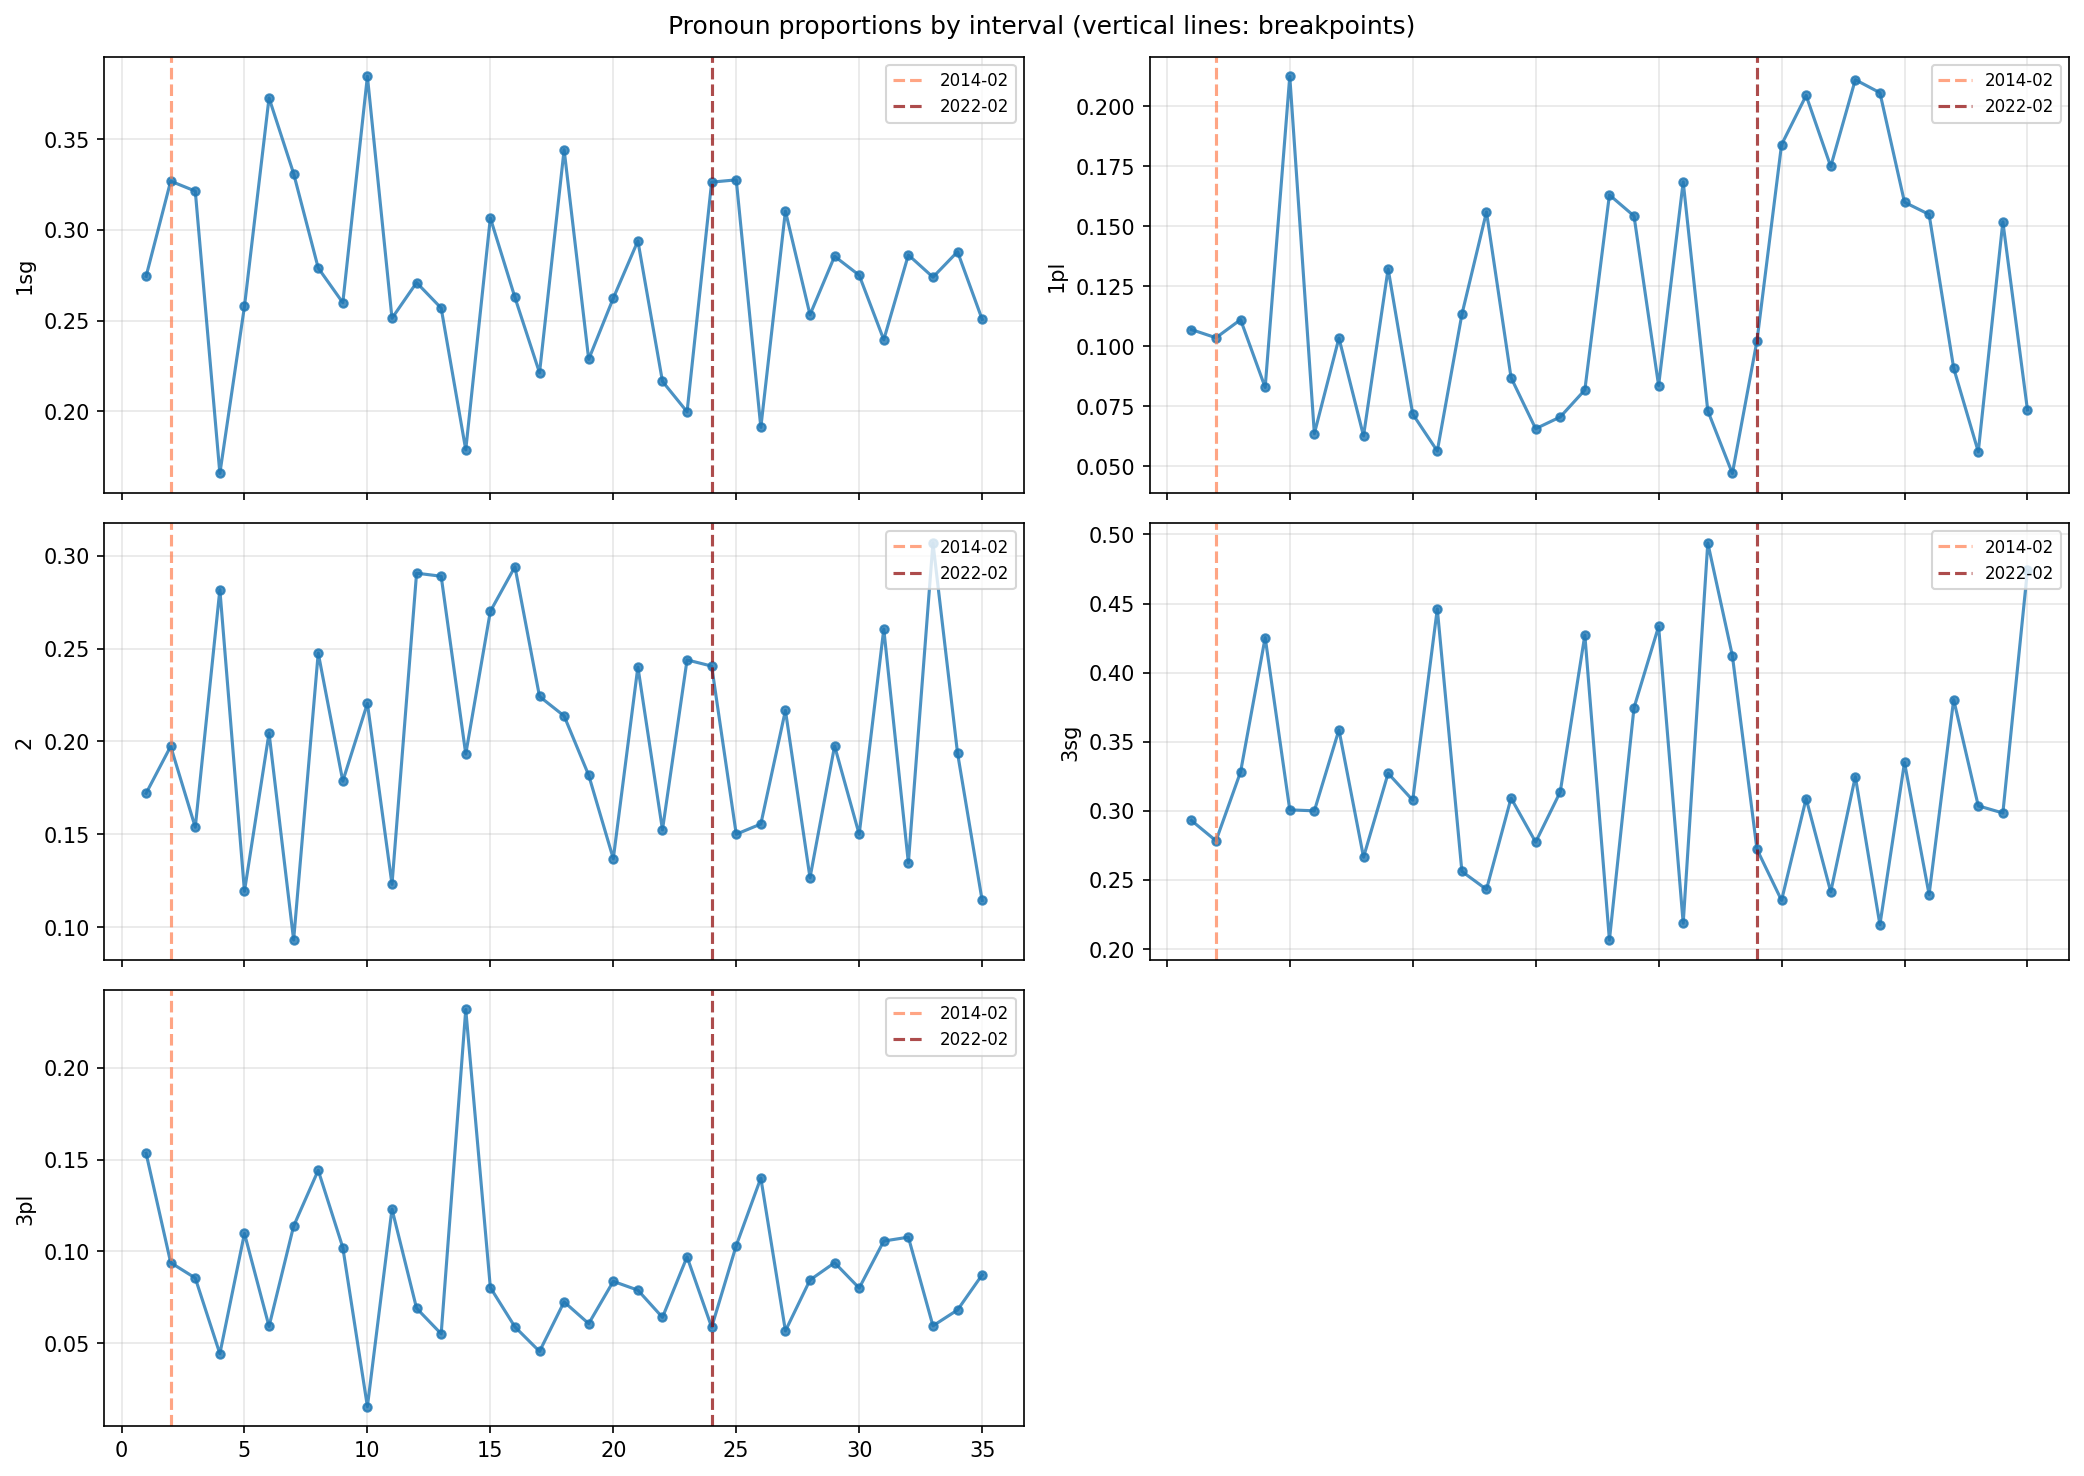
\includegraphics[width=0.95\textwidth]{fig1_breakpoint_timeseries.png}
\caption{Adaptive temporal binning (35 bins, each with $\geq 30$ poems) of per-stanza pronoun rates over 2013--2025, with piecewise weighted-least-squares fits (knots fixed a priori at 2014 and 2022) and PELT-detected change-points marked. The 1pl trajectory exhibits a marginal level shift at the 2022 knot ($\hat{\beta} = +0.20$, $p = 0.051$) and two PELT change-points (2022-03-01, 2023-02-10) bracketing the invasion. 1sg shows a confirmed 2014 level shift but is stable across 2022. 2sg/2pl trajectories are null at both knots.}
\label{fig:rq1-breakpoint}
\end{figure}

Figure~\ref{fig:rq1-timeseries} replots the 1pl share at annual resolution within the closed quartet, stratified by language. The Ukrainian-language series is dense enough across the entire window (large solid dots) to support visual inference: the bootstrap-95\,\% ribbon widens after 2022 because the per-year poem count thins, but the central tendency is uniformly above the pre-2014 baseline and remains there through 2025. The Russian-language series is supported by $\geq 10$ poems per year only through 2022 (faded dots after); the post-2022 Russian-stratum trajectory should therefore be read against the small-$n$ caveat embedded in the figure rather than against the central-tendency line.

\begin{figure}[h]
\centering

\includegraphics[width=0.95\textwidth]{fig_narr_1_time_series_we_rises.png}
\caption{Annual mean 1pl share within the closed first/second-person quartet, 2013--2025, by language stratum. Large solid markers denote years with $\geq 10$ poems in the stratum; small faded markers denote sparse years (interpret cautiously). Shaded ribbons are bootstrap 95\,\% CI around the per-year mean. The vertical wine bar marks 24 February 2022.}
\label{fig:rq1-timeseries}
\end{figure}

\subsubsection{RQ1 summary}

Across both language strata and under both the Poisson and the negative-binomial specifications, no within-author cell-level rate shift across the 24 February 2022 cutpoint survives the BH-FDR confirmatory criterion at $\alpha = 0.05$. The 1pl point estimates are uniformly positive (Ukrainian: IRR $= 1.20$; Russian: IRR $= 1.08$; pooled: IRR $= 1.18$) and the true-plural \textukrainian{ви} estimates are uniformly negative, but the corpus-clustered standard errors and the wild-cluster bootstrap render every cell-level claim non-significant after multiplicity correction. The corpus-level mean therefore cannot be read as having undergone a homogeneous, statistically detectable post-invasion shift in any single pronoun cell; whether that null reflects the absence of an effect or the presence of countervailing author-level trajectories is the question that RQ2 addresses directly.

\subsection{Individual Author Trajectories and Heterogeneity (RQ2)}
\label{sec:results-rq2}

For each of the five pronoun cells \{1sg, 1pl, 2sg, polite-singular \textukrainian{ви}, true-plural \textukrainian{ви}\} and each language stratum, we fit a poem-level negative-binomial hierarchical model with an author-level random slope on the period indicator, four chains of 2{,}000 draws after a 2{,}000-iteration warm-up via NUTS in Bambi (PyMC backend), $\widehat{R} < 1.02$ across all monitored parameters. Inference is summarized by 95\,\% highest-density intervals (HDIs) and by the posterior probability of direction $\Pr(\delta > 0\,|\,\text{data})$, with BH-style $q$-direction control applied within each cell.

\subsubsection{Population-level period shift after partial pooling}

The hierarchical population-level shifts replicate the RQ1 null (Table~\ref{tab:rq2-pop}). All ten cell-by-stratum HDIs include zero; the smallest $q_{\text{direction}}$ in the pooled stratum is $0.41$ (1sg and 1pl), and the smallest in any stratum is $0.24$ (Russian 2sg). The hierarchical posteriors do, however, sharpen the directional reading of the RQ1 specification curve: the pooled-stratum 1pl population shift posterior places $76\,\%$ of mass above zero (posterior mean rate ratio $= 1.14$, $95\,\%$ HDI $= [0.77, 1.65]$), and the pooled true-plural \textukrainian{ви} shift sits at posterior mean rate ratio $1.06$ with HDI $[0.54, 2.01]$.

\begin{table}[h]
\caption{RQ2 population-level period shift (posterior summaries from the hierarchical NB random-slope model). All ten HDIs include zero; no cell carries $q_{\text{direction}} < 0.05$.}
\label{tab:rq2-pop}
\centering
\small
\begin{tabular}{llrrrr}
\toprule
Stratum & Cell & RR (post.\ mean) & HDI95 & $\Pr(\delta > 0)$ & $q_{\text{direction}}$ \\
\midrule
Pooled & 1sg & 0.88 & [0.64, 1.20] & 0.22 & 0.41 \\
Pooled & 1pl & 1.14 & [0.77, 1.65] & 0.76 & 0.41 \\
Pooled & 2sg & 0.90 & [0.66, 1.21] & 0.24 & 0.41 \\
Pooled & polite-sg.~\textukrainian{ви} & 0.79 & [0.20, 2.74] & 0.37 & 0.41 \\
Pooled & true-pl.~\textukrainian{ви} & 1.06 & [0.54, 2.01] & 0.59 & 0.41 \\
Ukrainian & 1sg & 0.96 & [0.70, 1.31] & 0.41 & 0.50 \\
Ukrainian & 1pl & 1.19 & [0.80, 1.74] & 0.81 & 0.48 \\
Ukrainian & 2sg & 0.84 & [0.62, 1.13] & 0.13 & 0.48 \\
Ukrainian & polite-sg.~\textukrainian{ви} & 0.97 & [0.21, 3.70] & 0.50 & 0.50 \\
Ukrainian & true-pl.~\textukrainian{ви} & 0.94 & [0.43, 1.95] & 0.45 & 0.50 \\
Russian & 1sg & 0.78 & [0.25, 1.92] & 0.29 & 0.29 \\
Russian & 1pl & 1.41 & [0.55, 3.18] & 0.80 & 0.26 \\
Russian & 2sg & 1.57 & [0.86, 2.73] & 0.94 & 0.24 \\
Russian & polite-sg.~\textukrainian{ви} & 0.06 & [0.0003, 3.05] & 0.10 & 0.24 \\
Russian & true-pl.~\textukrainian{ви} & 1.73 & [0.44, 6.79] & 0.79 & 0.26 \\
\bottomrule
\end{tabular}
\end{table}

\subsubsection{Author random-slope variance}

The aggregate null masks substantial author-level heterogeneity. In the pooled stratum, the posterior standard deviation of the author-level period-shift deviation (i.e.\ each author's offset from the population mean on the log-rate scale) is $\sigma_{\delta} = 0.50$ for 1sg, $0.56$ for 1pl, and $0.53$ for 2sg, magnitudes comparable to the population mean itself. On the rate-ratio scale, individual authors range from $\mathrm{RR} = 0.42$ to $\mathrm{RR} = 4.70$ on the 1pl cell, with the highest five posterior means clustered around authors who took on documented frontline or combat-medic roles after February 2022 (Mitrov $4.70$, Kiva $2.97$, Chornohuz $2.78$, Zharikova $2.57$, Khersonsky $2.00$; all five carry $\Pr(\delta > 0\,|\,\text{data}) > 0.96$) and the lowest three clustered around older Kyiv-resident poets who curtailed posting or evacuated in 2022 (Babkina $0.42$, Andrusiak $0.43$, Falkovych $0.43$; all three carry $\Pr(\delta > 0\,|\,\text{data}) < 0.11$). Two authors in the pooled stratum have a 1pl deviation HDI that excludes zero in the positive direction and one has $q_{\text{direction}} < 0.05$; none has a negative-direction HDI excluding zero.

The 2sg cell is the only one in which posterior heterogeneity runs in both directions: three authors carry positive 2sg deviation HDIs excluding zero and three carry negative ones, with two passing $q_{\text{direction}} < 0.05$. The 1sg cell is dominantly negative on the population mean (RR $= 0.88$) but its author-level posteriors include two strongly positive outliers (HDI excluding zero, $q_{\text{direction}} < 0.05$ for one), consistent with a small subset of poets shifting more weight onto the lyric ``I'' even as the corpus mean drifts the other way.

Figure~\ref{fig:rq2-trajectories} displays each roster author's pre-2022 position in the (1sg-share, 1pl-share) plane of the closed quartet together with an arrow to their wartime position. Pale-cream arrows show the full roster; eight narratively notable authors are highlighted in literary red (female) and dark teal (male) with leader-line labels. The cloud of arrows visibly disperses rather than coheres: a small high-mobility cluster (Mitrov, Kiva, Chornohuz, Zharikova) translates simultaneously up in the 1pl axis and left in the 1sg axis, while a separate cluster (Falkovych, Babkina, Andrusiak) drifts in the opposite direction. The displacement structure is the geometric counterpart of the random-slope variance reported in the preceding paragraph.

\begin{figure}[h]
\centering

\includegraphics[width=0.98\textwidth]{fig_narr_2_author_trajectories.png}
\caption{Author trajectories in the (1sg-share, 1pl-share) plane of the closed first/second-person quartet. Each arrow runs from the author's pre-2022 mean position (dot) to their wartime position (arrowhead). Faded cream arrows: full roster ($n = 33$). Highlighted colored arrows: eight narratively notable authors (female: burgundy, male: deep teal). Dashed grey diagonals mark constant total-1st-person share isolines.}
\label{fig:rq2-trajectories}
\end{figure}

\subsubsection{Polite-singular \texorpdfstring{\textukrainian{ви}}{vy} under partial pooling}

The polite-singular \textukrainian{ви} cell exemplifies the rationale for the Bayesian path. Only 23 polite-singular tokens are observed across the entire roster, spread across 18 poems and 13 authors; only three authors contribute polite-singular tokens in both the pre-2022 and the post-2022 periods. Under maximum likelihood (the frequentist RQ1 path), this cell is therefore dropped: separation and zero within-author variance make the period coefficient and its standard error uninterpretable. The hierarchical NB resolves the same data through partial pooling: every author's posterior is shrunk toward the corpus-wide population mean by a factor proportional to the inverse of their observed information. As a consequence, the standard deviation of the polite-singular author deviation collapses to $\sigma_{\delta} = 0.23$ (vs.\ $0.50$--$0.56$ on the open cells), the author-level total period-shift rate ratios are tightly bounded to the interval $[0.64, 1.56]$ across all 33 authors, and no author carries a polite-singular deviation HDI excluding zero. The polite-singular posteriors are wide but coherent: the population mean rate ratio is $0.79$ (HDI $[0.20, 2.74]$, $\Pr(\delta < 0) = 0.63$), consistent with a directional retreat from the formal-singular register but not with a confirmatory claim.

\subsubsection{Caterpillar of the 1pl per-author posterior}

Figure~\ref{fig:rq2-caterpillar} displays the per-author posterior total period-shift on the 1pl cell in the pooled stratum, the cell that hosts the strongest cross-author dispersion identified in \S~\ref{sec:results-rq2}. Authors are sorted by posterior mean total shift (most positive at top, most negative at bottom); the top-five and bottom-five authors are colored in the literary palette and labelled with their posterior-mean rate ratio, while the middle band of $23$ authors is greyed as context. The figure is restricted to the 1pl cell deliberately, both to fit a single printed page with named author labels and to focus the visual on the cell that carries the manuscript's heterogeneity finding. The four remaining cells display qualitatively similar dispersion patterns; their analogous caterpillars are produced by the modeling script and are reported in the supplementary material.

\begin{figure}[h]
\centering

\includegraphics[width=0.92\textwidth]{fig_narr_8_caterpillar_1pl_focused.png}
\caption{Per-author posterior total period-shift on the 1pl cell, pooled Ukrainian + Russian stratum. Each row is one author; thick segments are 95\,\% highest-density intervals; the thin vertical at zero marks the no-shift null; the dashed vertical marks the across-author population mean. Top-five authors (deep-teal) and bottom-five authors (burgundy) are labeled with their posterior-mean rate ratio; the middle band of $23$ authors is greyed for context. The secondary upper axis re-expresses the log-rate shift on the multiplicative rate-ratio scale.}
\label{fig:rq2-caterpillar}
\end{figure}

\subsubsection{RQ2 summary}

The aggregate corpus-level null established by RQ1 conceals a heterogeneous, biographically-conditioned distribution of author-level trajectories. The 1pl cell hosts a cluster of strongly positive shifts among poets with documented post-2022 civic or military roles and a parallel cluster of negative shifts among older Kyiv-resident poets and post-2022 evacuees; the 2sg cell is uniquely bidirectional; and the polite-singular \textukrainian{ви} cell, on which the frequentist analysis is uninformative, is rendered interpretable through partial pooling at the cost of compressed individual posteriors. The population-level posteriors return the same null pattern as the frequentist GLMs (Table~\ref{tab:rq2-pop}), but the author-level posteriors document substantial cross-author variance that the corpus mean integrates out.

Figure~\ref{fig:rq2-cases} unpacks the author-level finding for six poets selected to span the heterogeneity reported above. Each panel plots the named poet's per-year 1pl share in the closed quartet with the 24 February 2022 cutpoint marked. The three frontline/combat-medic poets in the top row (Mitrov, Kiva, Chornohuz) and Serhiy Zhadan in the lower-left panel exhibit visible step-ups across the cutpoint; Boris Khersonsky shows a delayed wartime spike concentrated in 2023; Hryhoryi Falkovych's per-year 1pl rate falls and his archive entries thin after 2022, consistent with the negative posterior tail. The six per-year trajectories anchor the population posteriors (Table~\ref{tab:rq2-pop}) and the random-slope deviation summaries (\S~\ref{sec:results-rq2}) to specific, traceable individual records.

\begin{figure}[h]
\centering

\includegraphics[width=0.98\textwidth]{fig_narr_5_case_study_poets.png}
\caption{Per-year 1pl share within the closed first/second-person quartet for six poets selected from the random-slope posteriors. Each panel is one poet; vertical wine bar marks 24 February 2022; small grey numbers above each dot are the poem count in that year. Biographic taglines beneath each title summarize the wartime context that the panel records.}
\label{fig:rq2-cases}
\end{figure}

\section{Discussions}

\subsection{Synthesis: heterogeneous reaction, not homogeneous crystallization}
\label{sec:discussion-synthesis}

The two analyses converge on a single empirical claim. The 24 February 2022 cutpoint does not produce a homogeneous corpus-level linguistic shift in any individual person--number cell: under the confirmatory criterion of agreement between Poisson and negative-binomial GLMs plus wild-cluster bootstrap survival of BH-FDR control, no cell in either the Ukrainian or the Russian language stratum reaches significance, and the hierarchical Bayesian replication returns a parallel null at the population level (Table~\ref{tab:rq2-pop}). The same data, partitioned at the author level, document substantial heterogeneous variance: random-slope standard deviations on the open cells range from $0.50$ to $0.56$ log-units, with individual author period-shifts spanning approximately three log-units on the 1pl cell alone, and with both ends of the 2sg distribution populated by HDI-excludes-zero authors. The core empirical tension is therefore not between a wartime shift and a peacetime status quo, but between two scales of measurement: the corpus mean is null, the author panel is dispersed, and the heterogeneity is structured rather than random. The strongest positive 1pl shifts cluster among poets who took on documented civic-military roles after 2022 (Mitrov, Chornohuz, Zharikova, Kiva, Khersonsky), and the strongest negative 1pl shifts cluster among older Kyiv-resident poets and post-2022 evacuees (Babkina, Andrusiak, Falkovych). The invasion did not crystallize a single shared wartime ``we''; it polarized the deictic field along biographical lines that the corpus mean dissolves.

\subsection{Theoretical callbacks}
\label{sec:discussion-theory}

\subsubsection{1PL shifts: Billig, Brubaker, and groupness as event}

\citet{billig1995banal}'s account of national flagging predicts that an existential rupture should increase the rate of banal, unreflective 1PL deixis among speakers who continue to operate within the imagined community. The RQ1 specification curve recovers exactly this directional signal (1pl is positive in $100\,\%$ of Ukrainian-stratum specifications and in the pooled stratum), but the magnitude does not survive BH-FDR correction. Read against the corpus mean, the wartime ``we'' is flagged but not statistically detectable as a corpus-level rate shift. Read at the author level, however, the strong positive 1pl posteriors concentrate not on the banal background of Ukrainian-language poetic discourse but on a specific subset of poets whose biographies underwent a categorical reclassification in 2022. This is precisely the reading licensed by \citet{brubaker2004ethnicity}'s reformulation of groupness as a contingent event: nationhood is not a property of the population but an achievement of categorization, mobilization, and discursive practice that some actors enact more intensively than others. \citet{brubaker2000beyond}'s decomposition of ``identity'' into identification, self-understanding, and commonality maps directly onto the RQ2 author panel: identification with the wartime collective is unevenly distributed even within a self-selected literary roster, and the 1pl rate is the trace that distribution leaves in the corpus.

Figure~\ref{fig:disc-cohort} disaggregates the four-cell quartet by generation cohort to make the same point structurally. Across all five cohorts the four-cell composition is approximately stable for 1sg, 2sg, and true-plural \textukrainian{ви} from pre-2022 to wartime; the only cohort that registers a visibly larger 1pl share within the post-2022 panel is the $1990\text{s}$ cohort (the youngest fighting-age cohort in the roster), whose 1pl share more than doubles ($9\,\% \to 20\,\%$ within the closed quartet). The pre-1970 and 1970s cohorts show no comparable shift; the 1980s cohort moves very modestly. The cohort-conditional reading is consistent with \citet{onuch2022the}'s account of post-2022 civic Ukrainian identity as a generation-specific performative achievement: the wartime ``we'' that the corpus mean does not detect is concentrated in the cohort whose biographies were most directly reconfigured by the invasion.

\begin{figure}[h]
\centering

\includegraphics[width=0.98\textwidth]{fig_narr_4_generation_cohort_composition.png}
\caption{Cohort-by-period composition of the four-cell first/second-person attention quartet, roster authors only. Each pair compares pre-2022 (top bar) vs.\ post-2022 (bottom bar) corpus composition for one generation cohort. Cohort labels appear in the left margin; sample sizes (authors $\cdot$ poems) are inset on each bar. Cell colors: 1sg (slate), 1pl (rust), 2sg (gold), true-plural \textukrainian{ви} (forest). The 1990s cohort is the only one whose 1pl share more than doubles after the invasion.}
\label{fig:disc-cohort}
\end{figure}

\subsubsection{Bidirectional 2sg and the wandering ``we''}

The 2sg cell is uniquely bidirectional in the random-slope posteriors: three authors increase intimate ``you'' usage post-2022 with HDIs excluding zero, and three decrease it. \citet{petersoo2007what}'s diagnosis of the ``wandering we'' anticipates this pattern at the level of pragmatic theory: the deictic center of national address is not a single fixed referent but oscillates among multiple in-group constructions, and pronominal choice indexes that oscillation. The wartime data extend Petersoo's claim from the 1PL axis (where her analysis was developed) onto the 2P axis: some poets pivot from intimate addressee construction (``thou, my reader'') toward collective address (``you, my country''), while others retain or intensify the intimate-elegiac register against the wartime background. \citet{papacharissi2015affective}'s account of networked structures of feeling provides the meso-level framework: Facebook-circulated wartime poetry functions as an affective public in which multiple incommensurable affect-loadings (mobilizational, mournful, militarized, lyric-introspective) circulate in parallel rather than coalescing into a single voice. \citet{lokot2018iamnotafraidtosayi, lokot2021beyond}'s concept of augmented dissent describes a similar discursive logic in adjacent online testimonial genres: short, first-person, affectively charged posts assembling into networked counter-publics whose constitutive unit is the individual stance, not the aggregated mean. The RQ2 caterpillar (Figure~\ref{fig:rq2-caterpillar}) is a quantitative analog of that structure: each row is one stance, and the panel is the public.

\subsubsection{Sociolinguistic grounding: Kulyk, Onuch, and the post-2022 civic identity}

\citet{kulyk2022imperfect, kulyk2024language} documents a historically sharp post-2022 retreat of Russian from everyday Ukrainian language practice and a corresponding rise of civic Ukrainian identifications that crosscut ethnolinguistic categories. \citet{onuch2022the} frames the post-2022 civic Ukrainian nation as a generation-specific, performative achievement that crystallized through the experience of invasion. The author-level pattern reported in \S\ref{sec:results-rq2} aligns with both accounts in the specific direction they would predict: the positive 1pl cluster is dominated by poets whose post-2022 biographies record an explicitly performative civic-military realignment (Mitrov enlisted in the 95th Air Assault Brigade in March 2022; Chornohuz served continuously as a combat medic in the 140th Marine Reconnaissance Battalion and received the 2024 Shevchenko Prize for that work; Zharikova has served as a Territorial Defence combat medic since February 2022; Kiva is documented displacement from Donetsk to Lviv with a coincident shift toward Ukrainian-language composition; Khersonsky is an Odesa-based Russian-language poet whose post-2022 publishing shifted into a bilingual register). The negative 1pl cluster is dominated by older Kyiv-resident poets and post-2022 evacuees whose archive entries thin substantially after 2022 (Falkovych b.~1940, evacuated to Kolomyia; Andrusiak b.~1968; Babkina b.~1985 with documented Kyiv-Warsaw circulation post-2022). The corpus-level null and the structured author-level dispersion are therefore consistent: the post-2022 civic Ukrainian ``we'' is not a uniform banal flag in this poetic field, it is the differential mobilization of specific biographically situated speakers, and the corpus mean inevitably averages mobilization against retreat.

Figure~\ref{fig:disc-map} projects the same heterogeneity onto the authors' region of birth. The Kyiv-born sub-roster ($n = 5$) is the only in-country region whose mean wartime $\Delta$1pl-share is negative, consistent with the Falkovych / Babkina / Andrusiak cluster. The East-Ukraine and South-Ukraine sub-rosters carry the largest positive mean shifts (\,$+8.3\,$pp and $+9.6\,$pp respectively), reflecting authors with the most direct biographical exposure to the front line. The off-map ``born abroad'' panel ($n = 2$; Maria Galina, Arkadii Shtypel) is more positive still ($+12.1\,$pp), driven by relocated bilingual poets whose post-2022 publication shifted in the same direction as the East-Ukraine in-country pattern. The geographic structuring is consistent with the Kulyk/Onuch civic-identity framing: the wartime ``we'' is concentrated in those biographies for which the invasion was, in the most concrete sense, a re-categorization of their own ground.

\begin{figure}[h]
\centering

\includegraphics[width=0.95\textwidth]{fig_narr_3_ukraine_birthplace_map.png}
\caption{Stylized tile map of Ukrainian sub-regions colored by the mean post-2022 minus pre-2022 change in the 1pl share within the closed quartet, computed over roster authors born in that sub-region. Side panel: off-map cohorts (born abroad). Diverging colorscale: cool tones $=$ wartime decline in 1pl share; warm tones $=$ wartime growth. Author counts inset on each tile.}
\label{fig:disc-map}
\end{figure}

\subsection{Methodological contribution}
\label{sec:discussion-contribution}

The findings above rest on a pipeline that joins two methodological pieces, neither of which is by itself novel but whose combination addresses a problem that has limited computational pronoun analysis in pro-drop languages: how to count what isn't there. Ukrainian and Russian, in common with most Slavic, Romance, and East-Asian languages, license null subjects whenever the referent is recoverable from verb morphology, and the missing subjects, in those languages, are systematically and overwhelmingly the first and second person, i.e.\ exactly the cells on which the present analysis turns. Surface tokenizers and rule-based morphological parsers cannot recover those omitted subjects; any count built on them undercounts 1P and 2P forms, and the undercount almost certainly varies by author, period, and register in ways that confound exactly the contrast of interest. We resolve this with a two-step LLM annotation that translates each stanza into Shakespearean English (whose obligatory explicit subjects and thou/ye T--V split provide a near-one-to-one mapping for the Ukrainian deictic inventory) before extracting pronoun counts from the translated surface form. The result is a pronoun inventory that recovers pro-dropped subjects rather than treating them as noise, and that preserves the polite-singular vs.\ true-plural distinction that surface-form parsers collapse.

The second piece is the within-author panel design. Treating each poet as their own control eliminates the between-author confounding that any cross-sectional analysis of literary corpora must otherwise contend with: differences in style, register, theme, training, language preference, and biographical context are absorbed into the author fixed effect (frequentist path) or the author random intercept (Bayesian path), and the period coefficient is identified from within-person change alone. The two-level architecture that pairs the per-cell frequentist GLM (RQ1) with the cell-by-author hierarchical NB (RQ2) is the empirical engine of the heterogeneous-reaction finding above: RQ1 establishes the corpus-level null under multiplicity control, RQ2 documents the structured author-level variance that the null integrates over, and the contrast between the two is what licenses the substantive claim that the invasion polarized rather than homogenized the deictic field.

For Computational Social Science and Digital Humanities, the contribution of the combined pipeline is threefold. First, the LLM pro-drop pass demonstrates that morphologically rich pro-drop languages are no longer outside the reach of quantitative pronoun analysis: the same person--number contrasts that have grounded decades of English-language political-discourse work are now available, at scale, for Ukrainian and (with equivalent prompt engineering) for the larger Slavic-Romance-East-Asian space. Second, the within-author panel design ports econometric within-person identification into a literary corpus: each poet contributes their own pre/post contrast, the corpus aggregates those contrasts under multiplicity control, and the hierarchical layer recovers the heterogeneity that the aggregate suppresses, a workflow that translates with minimal adaptation to any longitudinal author-keyed corpus (legislative speeches, judicial opinions, autobiographical memoir, journalistic columns). Third, the two-level RQ1/RQ2 architecture demonstrates that homogeneous- and heterogeneous-effect tests are complementary rather than competing: a corpus that reads as null on the mean can simultaneously document substantial structured heterogeneity at the individual level, and the literary-studies and political-pragmatic readings of that heterogeneity (in the present case, the post-2022 polarization of the Ukrainian poetic ``we'') depend on having both layers in evidence rather than choosing between them.

\section{Conclusions}

\section{Limitations}

\section*{Acknowledgment}

An unnumbered section, e.g.\ \verb"\section*{Acknowledgements}", may be used for thanks, etc.\ if required and included \emph{in the non-anonymous version} before any Notes or References.


\section*{Disclosure statement}

An unnumbered section, e.g.\ \verb"\section*{Disclosure statement}", may be used to declare any potential conflict of interest and included \emph{in the non-anonymous version} before any Notes or References, after any Acknowledgments and before any Funding information.

\bibliographystyle{tfcad}
\bibliography{reference}

\appendix

\section{Roster sample composition}
\label{app:sample}

Figure~\ref{fig:app-sample} reports the cell-by-level frequencies of the four time-invariant author-level covariates used in the RQ2 random-slope model (gender, generation cohort, region of birth, and empirical period-1 language), restricted to the $33$ roster authors who enter the modeled sample. The figure documents the composition that the population-level posteriors in Table~\ref{tab:rq2-pop} integrate over and that the biographical clustering in \S\ref{sec:discussion-theory} reads against. The roster is gender-balanced ($14$ female, $19$ male, $1$ undeclared), generationally concentrated in the 1980s cohort ($n = 13$) and the pre-1970 cohort ($n = 9$), regionally over-weighted to West-Ukraine ($n = 14$) and Kyiv / East-Ukraine ($n = 5$ each), and linguistically dominated by Ukrainian-primary writers ($n = 27$) over Russian-primary writers ($n = 6$).

\begin{figure}[h]
\centering

\includegraphics[width=0.98\textwidth]{fig_narr_6_roster_sample_composition.png}
\caption{Counts of authors in the modeled roster by each time-invariant covariate used in the RQ2 covariate-adjusted sensitivity layer ($n_{\text{authors}} = 33$). The four panels (gender, generation cohort, region of birth, empirical period-1 language) are the same factors that enter the hierarchical model in \S\ref{sec:results-rq2} and that anchor the biographical interpretation in \S\ref{sec:discussion-theory}.}
\label{fig:app-sample}
\end{figure}

\end{document}
